%!TEX root = ../dissertation.tex

\chapter*{Preface}
\addcontentsline{toc}{chapter}{Preface}
\label{chap:preface}

\Lettrine{Scientific} progress is tightly linked to human curiosity, a driving force that has brought us further and further every decade. The same impulses that thrusted imagination into wondering what those lights in the sky are, kept us on Earth trying to figure out how far we can get splitting matter into pieces. A mountain can be reduced to rocks, stones, pebbles, sand, dust and$ \ldots $  where do we stop? That question gave birth to the \textit{atomism} philosophy in Ancient Greece, when the term for the modern word \textit{atom} was coined: \textit{ἄ$\tau$ο$\mu$ο$\nu$ (atomon, indivisible)}. In atomism, all matter is composed of atoms and void. Those philosophical atoms, in all shapes and sizes, could collide with each other or hook together to form clusters resulting in their observable, macroscopic counterparts or \textit{substances}.

\textit{Atomism} was just a philosophical current trying to explain the world without any empirical observations to prove those hypotheses. It can be considered the first atomic model; albeit a useless one. This does not necessarily mean it is a bad model. Models are \textbf{simplifications of reality that can provide explanations and predictions of reproducible observations}. In this case, atomism failed to explain actual phenomena, but did satisfy the philosophical curiosity behind its inception. As a result, one can only assess the quality of a model in terms of its purpose: it will be valid as long as this is fulfilled (see fig. \ref{fig:penicillin}).



\begin{figure}[H]
	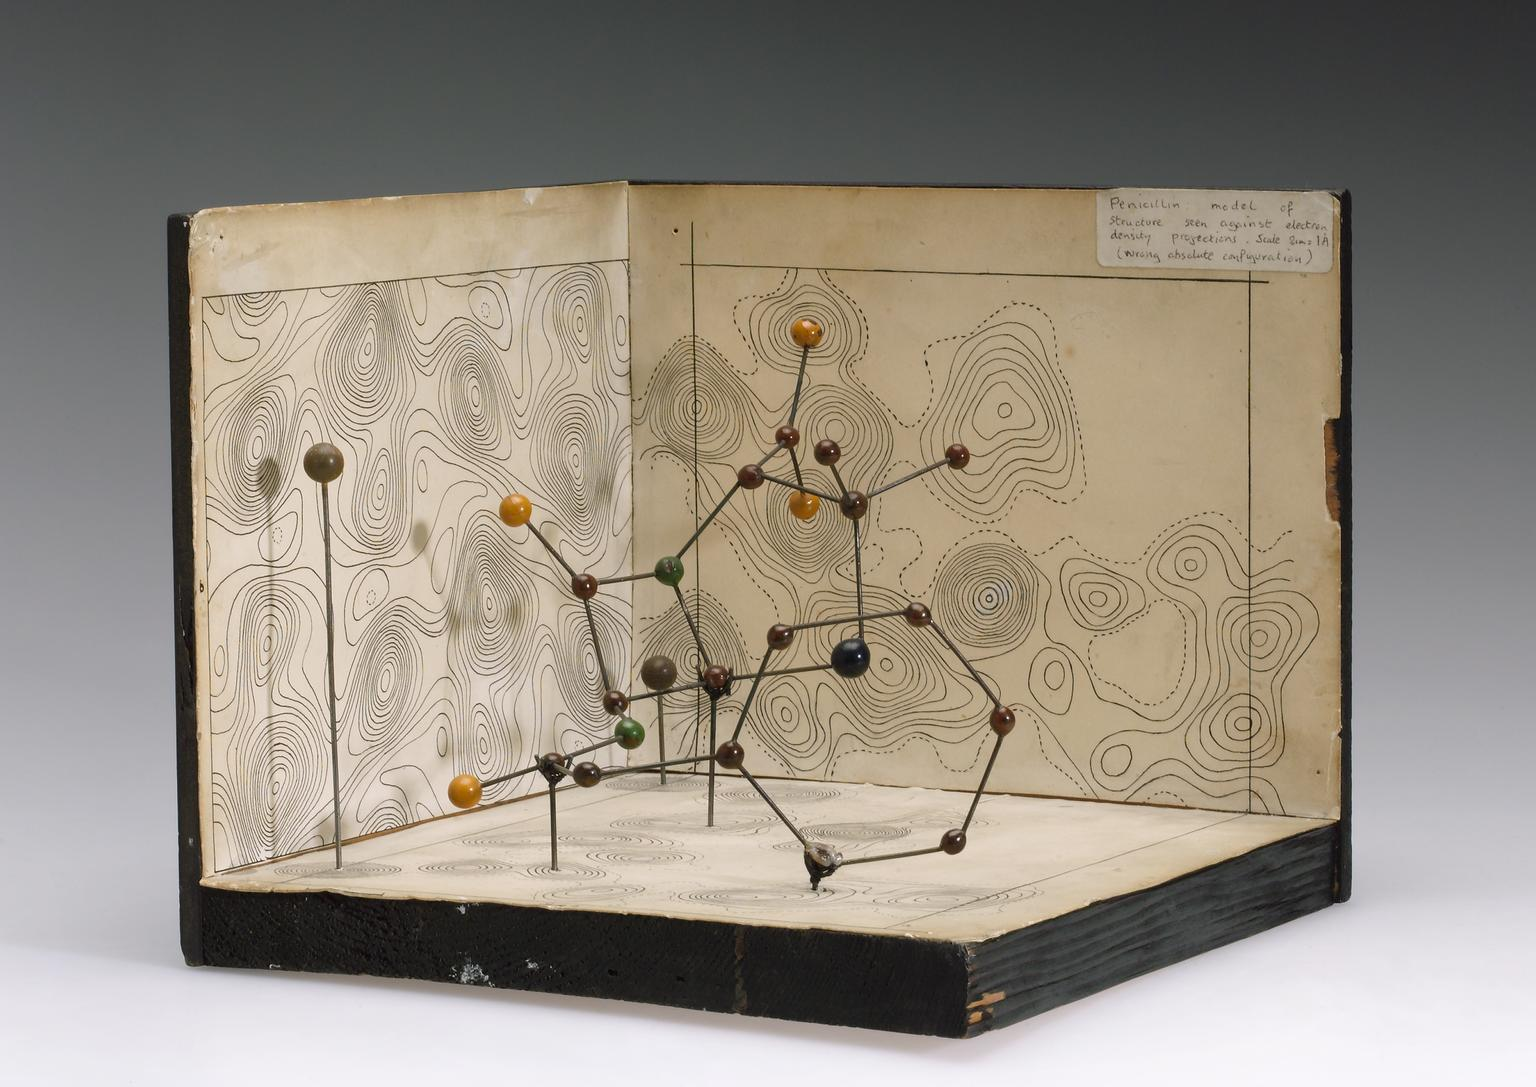
\includegraphics[width=\textwidth]{./figures/01/penicillin.jpg}
	\caption[Dorothy M. Crowfoot's 1945 Penicillin model]{In the pre-computer era, models were built physically. Here depicted, Dorothy M. Crowfoot's 1945 penicillin model. Reproduced from UK's Science Museum $ \{ $ uksciencemuseum $ \} $.}
	\label{fig:penicillin}
\end{figure}


Since the clusters described by atomism do not provide useful predictions on molecules, new models have been described over the past decades, each replacing the previous one to address new conflicting observations: Dalton, Thomson, Rutherford, Bohr$ \ldots $ \  During the past century, we have seen the atom acquiring unthought complexity: nuclei, electrons, protons, neutrons, quarks$ \ldots $  Harnessing this complexity in a new model does not mean that we always use the most sophisticated theories. Sometimes, it is simply overkill and unnecessary. The same way relativistic effects are not considered during the preparation of a cheesecake, quantum effects can be ignored in some types of studies. Other times, they must be considered, though.

The complexity of the underlying theory of a model usually correlates with the mathematical principles behind, so the more complex a model becomes, the harder it is to apply it. Even if the model itself it is not mathematically complex, the accumulated steps to obtain a satisfactory answer can make it costly. Fortunately, the uprising of computation in last decades has greatly eased the resolution of the equations proposed by the advances in theoretical chemistry. In fact, the marriage of modeling and computation is so widespread that when one says ‘modeling’, it is commonly understood as ‘computational modeling’.